\documentclass[12pt,oneside]{book}

\usepackage[dvips,letterpaper,margin=0.75in,bottom=0.5in]{geometry}
\usepackage{cite}
\usepackage{slashed}
\usepackage{graphicx}
\usepackage{amsmath}
\usepackage{braket}
\usepackage{multicol}

\begin{document}

\title{Analysis of Experimental Data}
\author{Michael Mulhearn}

\maketitle

\chapter{Statistical Distributions}

\section{Notes on Section Ordering}

To reach Section~\ref{sec:comphist} as rapidly as possible, delay
Sections~\ref{sec:poisson} and \ref{sec:poissonmeanvar} and delay or
even skip \ref{sec:gaussfrompoisson}.

\section{Statistics of Experiments}

A primary purpose of science is to predict the results of experiments.
Consider a simple experiment with five possible outcomes which we
repeat ten times.  If our theoretical prediction is that each of these
five outcomes is equally probable, than our prediction for a typical
series of ten experiments would be for each outcome to occur two
times.  Now suppose we perform the experiment ten times and present
the results like this:

\begin{figure}[htbp]
\begin{center}
{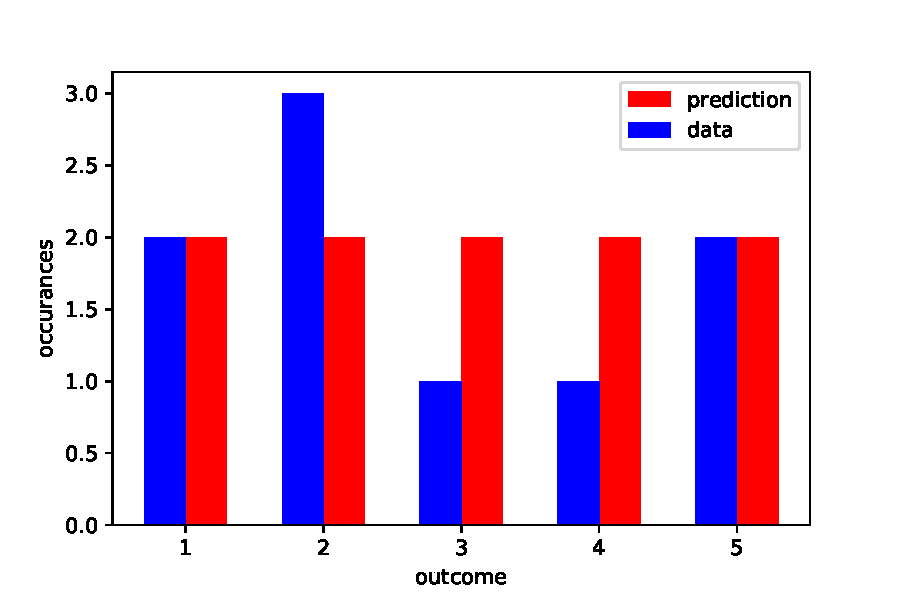
\includegraphics[width=0.45\textwidth]{figs/intro.pdf}}
\end{center}
\caption{\label{fig:intro} Comparison of experimental results with a prediction.}
\end{figure}

Scientist almost never display experimental data this way (as a bar
graph) because it is nearly impossible to answer the crucial question
{\em is this data consistent with this prediction?}  Even if every
outcome has an equal probability, the measured results of individual
experiments will result from random statistical fluctuations.  So even
if the theory is correct, we well seldom reproduce exactly the theory
prediction.

To interpret scientific experiments, it isn't enough to have a single
prediction for the outcome of an experiment, instead, you need a
prediction for the statistical distribution of outcomes.  The
mathematical framework for providing this prediction is called a
probability distribution, which reports the probability of each
possible outcome for a random variable.  We'll start this discussion,
therefore, by deriving three of the most frequently encountered
probability distributions: the Binomial Distribution, the Poisson
Distribution, and the Gaussian Distribution.


\section{The  Binomial Distribution}

The Binomial Distribution is the most general of the distributions
we'll consider, but it is a bit cumbersome to use in practice.  The
more familiar Poisson and Gaussian distributions are limiting cases of
this distribution.

\begin{figure}[htbp]
\begin{center}
\begin{tabular}{cc}
{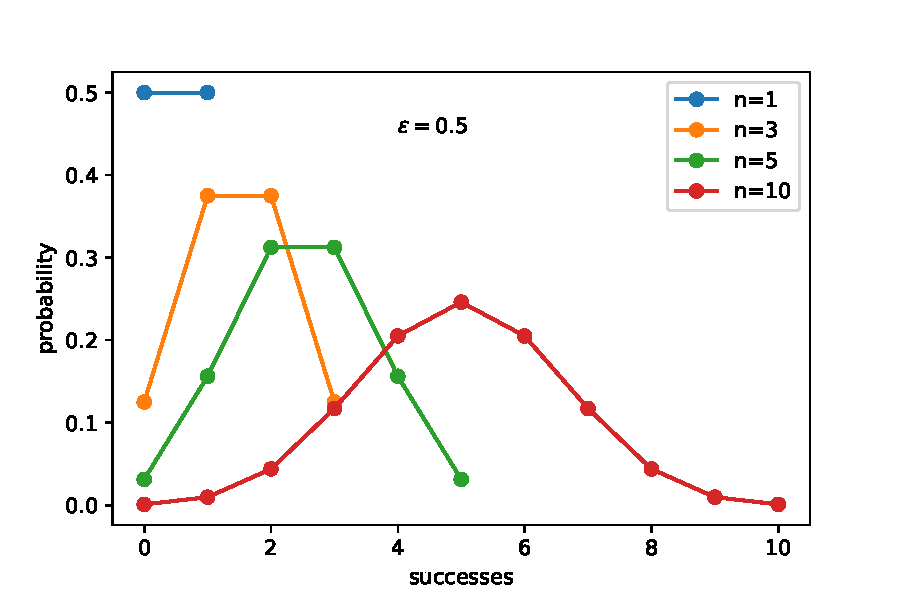
\includegraphics[width=0.47\textwidth]{figs/binom_n.pdf}} &
{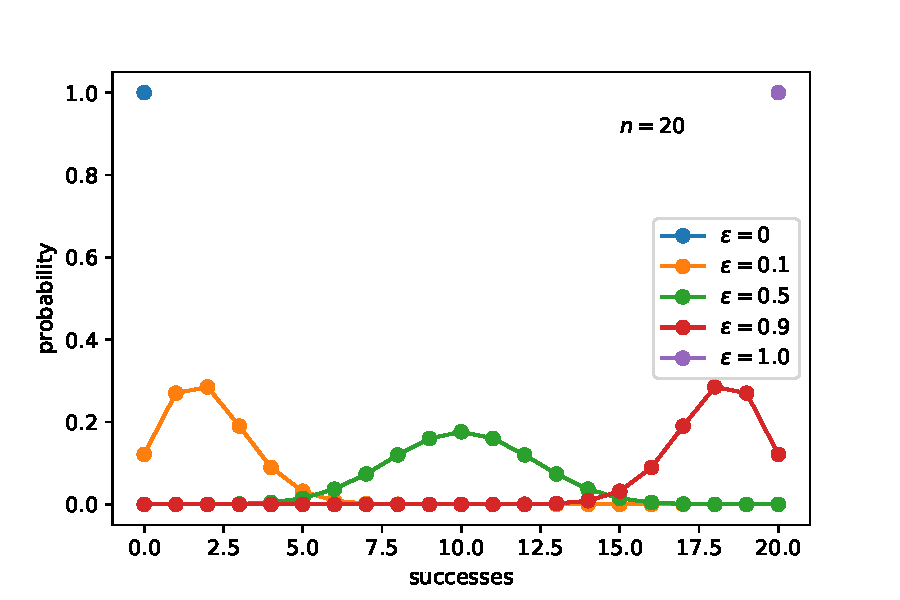
\includegraphics[width=0.47\textwidth]{figs/binom_eps.pdf}} \\
(a) & (b) \\
\end{tabular}
\end{center}
\caption{\label{fig:binom} The binomial distribution for several different values of the parameters (a) $n$ and (b) $\epsilon$.}
\end{figure}

Suppose you repeat a particular process $n$ times, and each time you
have the same probability $\epsilon$ of a particular outcome, which,
without losing generality, we'll call ``success".  The probability of
having exactly $m$ successes after $n$ trials is simply given by:
\begin{displaymath}
P = \sum_i p_i
\end{displaymath}
where $i$ runs over all specific outcomes with $m$ successes and $p_i$
is the probability of each specific outcome.  However, as these
specific outcomes all contain exactly $m$ successes, they share the
same probability, namely:
\begin{displaymath}
p_i = \epsilon^m (1 - \epsilon)^{n-m}
\end{displaymath}
and so we are left to consider simply the total number of specific outcomes containing $m$ successes.  

The quantity we need is provided by the binomial theorem from mathematics, which states that:
\begin{equation}
\label{eqn:binomt}
(p+q)^n = \sum_{m=0}^{n} \binom{n}{m} \, p^m \, q^{n-m}
\end{equation}
where the binomial coefficients are defined by
\begin{equation}
\label{eqn:binomc}
\binom{n}{m} = \frac{n!}{m! \, (n-m)!}
\end{equation}
and are also often referred to in other contexts as $n$-choose-$m$.  The binomial coefficient simply tells us how many times we can choose $m$ instances of $p$ instead of $q$, from $n$ factors, and so it is precisely the combinatoric factor that we need.

The probability of obtaining $m$ successes after $n$ trials with probability $\epsilon$ is therefore given by:
\begin{equation}
\label{eqn:binom}
P(m; \, n ,\epsilon) = \binom{n}{m} \, \epsilon^m \, (1 - \epsilon)^{n-m}
\end{equation}
which is called the Binomial Distribution.

\section{Mean and Variance of a Probability Distribution}

Given a probability distribution describing the outcomes of an experiment, our
most urgent questions are generally ``what is a typical outcome?'' and ``how widely will outcomes typically vary from one another?''.

There are a number of ways to quantitfy the answer to first question,
but generally the most useful answer is the mean value, $\mu$, also called
the expected value, of the distribution, which is defined as the
weighted average across all possible outcomes.  For the Binomial distribution, which describes probabilities for outcomes which are natural numbers up to $n$, we calculate the sum:
\begin{equation}
\mu \equiv \braket{m} \equiv \sum_{m=0}^{n} m \, P(m)
\end{equation}
For a continuous probability distribution, where outcomes can be any
real value, we would integrate instead:
\begin{equation}
\mu \equiv \braket{x} \equiv \int_{-\infty}^{+\infty} x \, P(x) \, dx 
\end{equation}
across a range appropriate to the situation, typically $[-\infty,\infty]$.

A mode of a distribution is an outcome for which the probability is
maximal.  A median of a distribution is a value at which $50\%$ of
probability is at or below it and $50\%$ of probability is at or above
it.  Both of these quantities provide information about typical values
for a distribution, but they suffer the signficant defect that they
are not necessarily unique for a given distribution.

We usually answer the second question in terms of the variance, $\sigma^2$, of the distribution:
\begin{displaymath}
\sigma^2 \equiv \braket{(x-\mu)^2}
\end{displaymath}
Other answers have problems, e.g. $\braket{x-\mu}$ can be zero or nearly so, even for wide distributions, as long as it is symmetric.  You could fix this by calculating $\braket{|x-\mu|}$ but this is generally much harder to calculate, and less useful, than the variance.  For instance, it is left as an exercise to show that:
\begin{equation}
\label{eqn:varhw}
\braket{(x-\mu)^2} = \braket{x^2} -\braket{x}^2
\end{equation}
using the fact that $\mu$ is simply a number, and so $\braket{\mu} = \mu$.  We need only calculate $\braket{x}$ and $\braket{x^2}$ in order to determine the variance of a distribution.

\section{Mean and Variance of the Binomial Distribution}

The mean value of Binomial Distribution is given by:
\begin{eqnarray*}
\braket{m} &=& \sum_{m=0}^n \; m \, P(m) \\
&=& \sum_{m=0}^n \; m \, \binom{n}{m} \epsilon^m (1-\epsilon)^{n-m} \\
\end{eqnarray*}
which looks rather daunting!  The trick is to use the Binomial Theorem (\ref{eqn:binomt}) and define a function of two independent variables $p$ and $q$ given by:
\begin{displaymath}
f(p,q) = (p+q)^n = \sum_{m=0}^n \binom{n}{m} p^m q^{n-m}
\end{displaymath}
We then calculate:
\begin{displaymath}
\frac{\partial f}{\partial p} = n(p+q)^{n-1} = \sum_{m=0}^n m \binom{n}{m} p^{m-1} q^{n-m} \\
\end{displaymath}
and multiplying by $p$ we have:
\begin{displaymath}
np(p+q)^{n+1} = \sum_{m=0}^n m \binom{n}{m} p^m q^{n-m}
\end{displaymath}
which is true for any $p$ and $q$.  We now substitute the particular values $p=\epsilon$ and $q=1-\epsilon$ and find that:
\begin{displaymath}
n \epsilon = \sum_{m=0}^n m \binom{n}{m} \epsilon^m (1-\epsilon)^{n-m} \equiv \sum_{m=0}^n m P(m) = \mu
\end{displaymath}
So the mean value is given by:
\begin{equation}
\mu = n \epsilon
\end{equation}
or the total number of trials times the probability of success for each trial, a wholly plausible answer.

For the variance, we use a variation of the same trick, this time using the second partial derivative:
\begin{displaymath}
p^2 \cdot \frac{\partial^2 f}{\partial p^2} = n(n-1)p^2(p+q)^{n-2} = \sum_{m=0}^n m (m-1) \binom{n}{m} p^{m} q^{n-m} \\
\end{displaymath}
and again putting $p=\epsilon$ and $q=1-\epsilon$ to find that:
\begin{eqnarray*}
n(n-1)\epsilon^2 &=& \sum_{m=0}^n (m^2 -m) \binom{n}{m} p^{m} q^{n-m} \\[5pt]
&=& \sum_{m=0}^n (m^2 -m) P(m) \\[5pt]
&=& \braket{m^2-m} = \braket{m^2}-\braket{m}
\end{eqnarray*}
and as $\braket{m} = n \epsilon$ we have:
\begin{displaymath}
\braket{m^2} = n(n-1)\epsilon^2 + n \epsilon
\end{displaymath}
And so:
\begin{displaymath}
\sigma^2 = \braket{m^2} - \braket{m}^2 = n(n-1)\epsilon^2 + n \epsilon - n^2\epsilon^2
\end{displaymath}
or simply:
\begin{equation}
\sigma^2 = n \, \epsilon \, (1 - \epsilon)
\end{equation}
Note that if $\epsilon=0$ or $\epsilon=1$, there is only one outcome (all failures or all success) and so the variation is zero.

\section{The Poisson Distribution}
\label{sec:poisson}

\begin{figure}[htbp]
\begin{center}
{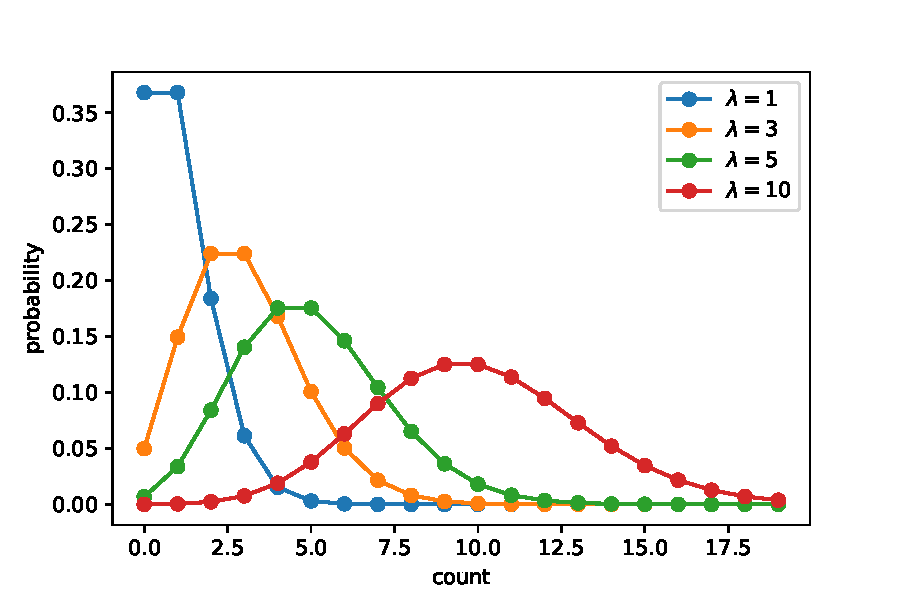
\includegraphics[width=0.45\textwidth]{figs/poisson.pdf}}
\end{center}
\caption{\label{fig:poisson}  The Poisson distribution for several values of parameter $\lambda$.}
\end{figure}

Suppose we have some time interval over which we expect to observe a
mean number of events $\lambda$.  The events must be independent of
one another: an event occurring at a particular time cannot affect the
time at which the next event occurs.  We divide the time interval over
which the $\lambda$ events are expected to occur into into $n$
sub-intervals, each with an equal probability to contain an event.
These intervals will be all the same size if the events are uniformly
distributed in time, but if the events are not uniformly distributed,
the sub-intervals are simply chosen to ensure the probability is the
same in each interval.  The probability of an event occuring in each
subinterval is $\epsilon = \lambda / n$.  If we make $n$ large enough,
the probability of observing two events in an interval is vanishing
small: $\epsilon^2 = \lambda^2 / n^2 \ll \epsilon$.  Once cast this way, we can
interpret the outcome of the counting experiment as drawn from a
Binomial distribution of $n$ trials each with $\epsilon = \lambda / n$:
\begin{eqnarray*}
P(m) &=& \binom{n}{m} \epsilon^m (1-\epsilon)^{n-m} \\[5pt]
  &=& \frac{n!}{m! \, (n-m)!} \; \left( \frac{\lambda}{n} \right)^m \left( 1 - \frac{\lambda}{n}\right)^{n-m} \\[5pt]
  &=& \left( \frac{\lambda^m}{m!} \right) \left(1-\frac{\lambda}{n} \right)^n \left[ \frac{n!}{(n-m)!} \cdot \frac{1}{n^m}\right]_1 \left[ \left( 1 - \frac{\lambda}{n}\right)^{-m}\right]_2
\end{eqnarray*}
We obtain the Poisson distribution by considering the limit that  $n \to \infty$.   It is left as an exercise to show that both $[\dots]_1 \to 1$ and $[\dots]_2 \to 1$ as $n \to \infty$.  Recalling that
\begin{displaymath}
\lim_{n \to \infty} \left(1 - \frac{\lambda}{n} \right)^n = e^{-\lambda}
\end{displaymath}
we obtain the Poisson distribution, the probability for observing $m$ events for a mean of $\lambda$:
\begin{equation}
\label{eqn:poisson}
P(m\; ; \; \lambda) = \frac{\lambda^m}{m!} \, e^{-\lambda}
\end{equation}
Notice that there is no longer a parameter $n$, since we took $n \to
\infty$, and so $m$ now ranges from 0 to $\infty$.  Note also that
$\lambda$ is a real number, not necessarily an integer, even though it
is the mean of integer values.  For example, the mean of the integers
1 and 2 is the real value 1.5.

\section{Mean and Variance of The Poisson Distribution}
\label{sec:poissonmeanvar}

The mean of the Poisson distribution is given by:
\begin{eqnarray*}
\mu &=& \sum_{m \geq 0} \; m \, P(m) \\
&=& \sum_{m \geq 0} \; m \, \frac{\lambda^m}{m!} \, e^{-\lambda}\\
\end{eqnarray*}
Since the first term ($m=0$) is zero, we have:
\begin{eqnarray}
\mu &=& e^{-\lambda} \sum_{m \geq 1} \; \frac{\lambda^m}{(m-1)!} \notag \\
             &=& \lambda e^{-\lambda} \sum_{m \geq 1} \; \frac{\lambda^{m-1}}{(m-1)!} \notag \\
             &=& \lambda e^{-\lambda} \sum_{n \geq 0} \; \frac{\lambda^{n}}{n!} \notag \\
             &=& \lambda e^{-\lambda} e^\lambda \notag \\
\mu  &=& \lambda
\end{eqnarray}
which should come as no surprise, as the assumption in the derivation was the that mean number of events was $\lambda$. 

For the variance, we use a similar manipulation to calculate:
\begin{eqnarray*}
\braket{m^2} &=& \sum_{m \geq 0} \; m^2 \, P(m) \\
&=& \sum_{m \geq 0} \; m^2 \, \frac{\lambda^m}{m!} \, e^{-\lambda}\\
&=& \lambda \sum_{m \geq 1} \; m \, \frac{\lambda^{m-1}}{(m-1)!} \, e^{-\lambda}\\
&=& \lambda \sum_{n \geq 0} \; (n+1) \, \frac{\lambda^{n}}{(n)!} \, e^{-\lambda}\\
&=& \lambda \braket{m+1} = \lambda \, (\lambda+1)
\end{eqnarray*}
And so:
\begin{eqnarray}
\sigma^2 &=& \braket{m^2} - \braket{m}^2 \notag \\
&=& \lambda \, (\lambda+1) - \lambda^2 \notag \\
\sigma^2 &=& \lambda. 
\end{eqnarray}
That is, the variance of a Poisson distribution is simply the mean.
This is probably the single most practical result from statistics.
Whenever a measurement amounts to a counting experiment, simply from
knowing the outcome of the experiment, the count $N$, we can estimate
that mean value $\mu \sim N$ and also the variance $\sigma^2 = N$.
Typical flutuations in a count $N$ are characterized by $\sigma =
\sqrt{N}$.

\section{The Gaussian Distribution}

\begin{figure}[htbp]
\begin{center}
{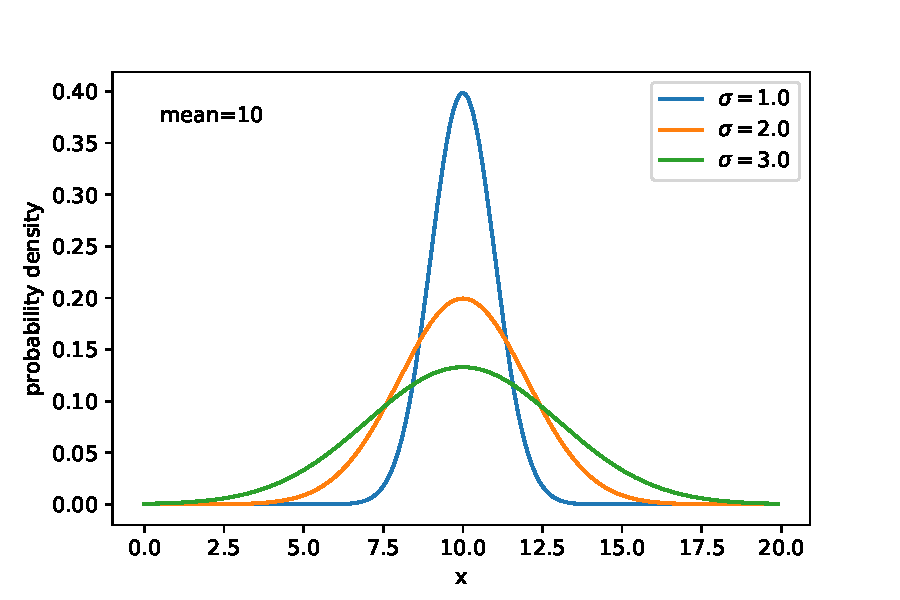
\includegraphics[width=0.45\textwidth]{figs/gaussian.pdf}}
\end{center}
\caption{\label{fig:gaussian}  The Gaussian distribution for a mean of 10 and several values of parameter $\sigma$.}
\end{figure}

The next distribution we will consider is the Gaussian distribution:
\begin{equation}
\label{eqn:gaussian}
P(x) = \frac{1}{\sqrt{2\pi} \sigma} \cdot \exp\left( - \frac{(x - \mu)^2}{2 \sigma^2}\right)
\end{equation}
which is plotted in Fig.~\ref{fig:gaussian}.  The Gaussian
distribution (often called the normal distribution) is the most
important and useful distribution as a consequence of the central
limit theorem (CLT).  The CLT states that when independent random
variables drawn from any distribution of finite variance are added
together and appropriately normalized (such as by taking their
average) the distribution of the resulting random variable approaches
the Gaussian distribution as the number of entries in the sum
increases to infinity.  A proof of the CLT is in the Appendix.

The Binomial and Poisson distribution are discrete functions: they
describes the probability of outcomes which are integer quantities.
For example, the Binomial probability for having 2.31 successes is
either undefined or taken to be zero.  The value of the
Binomial distribution function at a particular integer value is simply
the probability of that particular outcome.  To determine the
probability that an outcome is within a range of integers, say $m_1$
to $m_2$ the probability distribution function is simply added:
\begin{displaymath}
P = \sum_{m=m_1}^{m_2} P(m).
\end{displaymath}

The Gaussian distribution is a continuous function that describes the
probability {\em density} at each position $x$.  The probability of
any particular outcome, say $x=1.24323$, is vanishing small.  But the
probability that the value lies within a range of values is non-zero,
and is determined by integrating:
\begin{displaymath}
P = \int_{x_{\rm min}}^{x_{\rm max}} P(x;\lambda,\sigma) \, dx
\end{displaymath}
The Gaussian distribution is called a probability density function
(PDF).  A discrete probability distribution is sometimes referred to
as probability mass function (PMF), to draw upon an analogy with
physical mass and density: a PDF is probability per unit volume while
a PMF is simply a probability.

The Gaussian distribution is normalized so that:
\begin{displaymath}
\int_{-\infty}^{+\infty} P(x) \, dx = 1
\end{displaymath}
To determine the mean value of a function $f(x)$ we likewise integrate:
\begin{displaymath}
\braket{f(x)} \equiv \int_{-\infty}^{+\infty} f(x) P(x) \, dx = 1
\end{displaymath}
In particular the mean value of $x$ can be calculated by:
\begin{displaymath}
\braket{x} \equiv \int_{-\infty}^{+\infty} x P(x) \, dx 
\end{displaymath}
and:
\begin{displaymath}
\braket{x^2}  \equiv \int_{-\infty}^{+\infty} x^2 P(x) \, dx 
\end{displaymath}
We have defined the Gaussian distribution with the suggestive
parameters $\mu$ and $\sigma$.  It is left as an exercise to show
that indeed, the mean is $\mu$ and the variance is $\sigma^2$.


\section{The Gaussian Distribution as a Limiting Case}
\label{sec:gaussfrompoisson}

As expected from the Central Limit Theorem, the Poisson Distribution in the limit $\lambda \to \infty$
approaches the Gaussian distribution.  In this case, we can apply the Stirling Approximation:
\begin{displaymath}
\lim_{n \to \infty} n! = \sqrt{2 \pi n} \; e^{-n} \; n^n
\end{displaymath}
to the Poisson distribution as follows:
\begin{eqnarray*}
P(m) &=& \frac{\lambda^m}{m!} \, e^{-\lambda} \\[5pt]
 &\to& \frac{\lambda^m e^{-\lambda}}{\sqrt{2 \pi m} \; e^{-m} \; m^m} \\[5pt]
 &=& \frac{e^{m-\lambda}}{\sqrt{2\pi\lambda}} \left( \frac{\lambda}{m}\right)^{m+\frac{1}{2}}\\
\end{eqnarray*}
Now we consider a new variable $\delta$, defined by
\begin{displaymath}
\delta \equiv \frac{m-\lambda}{\lambda}
\end{displaymath}
which measures the difference between the observed number of events $m$ and the mean of the distribution, as a fraction of the mean.  Intuitively, the function is getting very narrow, and so we expect this to be a small quantity, but let's check this.  First we have:
\begin{displaymath}
\braket{\delta} = \frac{\braket{m}- \lambda}{\lambda} = \frac{\lambda - \lambda}{\lambda} = 0
\end{displaymath}
but also:
\begin{displaymath}
\braket{\delta^2} = \frac{\braket{(m-\lambda)^2}}{\lambda^2} = \frac{\lambda}{\lambda^2} = \frac{1}{\lambda}
\end{displaymath}
where we have used the fact that the variance is given by $\braket{(m-\lambda)^2} = \lambda$, and so as $\lambda \to \infty $ we have
\begin{displaymath}
\braket{\delta^2} \to 0
\end{displaymath}
So we can write:
\begin{equation} \label{eqn:mdef}
m = \lambda (1 + \delta)
\end{equation}
where we expect the approximation $\delta \to 0$ to hold as long as we require $\lambda \to \infty$.  So now we can write the distribution in terms of the small quantity $\delta$ and the large quantity $\lambda$ as:
\begin{eqnarray}
\label{eqn:pdelt}
P(\delta) &=& \frac{e^{\lambda\delta}}{\sqrt{2\pi\lambda}} \left( \frac{\lambda}{\lambda (1+\delta)} \right)^{\lambda(1+\delta)+\frac{1}{2}} \notag \\[5pt]
 &=& \frac{e^{\lambda\delta}}{\sqrt{2\pi\lambda}} \cdot \frac{1}{X}
\end{eqnarray}
where we define the quantity:
\begin{displaymath}
X = (1+\delta)^{\lambda(1+\delta)+\frac{1}{2}}
\end{displaymath}
which can be approximated as follows:
\begin{eqnarray*}
\ln X &=& \left( \lambda (1+\delta) + \frac{1}{2} \right) \cdot \ln(1+\delta) \\[5pt]
&=& \left( \lambda (1+\delta) + \frac{1}{2} \right) \cdot \left( \delta - \frac{\delta^2}{2} + \mathcal{O}(\delta^3)\right) \\[5pt]
\frac{\ln X}{\lambda}&=& \left( 1+\delta + \frac{1}{2\lambda} \right) \cdot \left( \delta - \frac{\delta^2}{2} + \mathcal{O}(\delta^3)\right) \\[5pt]
&=& \left( 1+\delta + \mathcal{O}\left(\delta^2\right) \right) \cdot \left( \delta - \frac{\delta^2}{2} + \mathcal{O}(\delta^3)\right) \\[5pt]
&=& \delta + \frac{\delta^2}{2}+ \mathcal{O}(\delta^3),
\end{eqnarray*}
where in the second to last step we used $\mathcal{O}\left(\frac{1}{\lambda}\right) \sim \mathcal{O}\left(\delta^2\right)$.  Neglecting the small quantities, we can approximate
\begin{displaymath}
X = \exp\left( \lambda\delta + \lambda\frac{\delta^2}{2} \right) 
\end{displaymath}
which, when plugged backed into Equation~\ref{eqn:pdelt} yields:
\begin{eqnarray}
\label{eqn:almost}
P(\delta) &=& \frac{e^{\lambda\delta}}{\sqrt{2\pi\lambda}} \cdot \frac{1}{\exp\left( \lambda\delta + \lambda\frac{\delta^2}{2} \right)} \notag \\[5pt]
&=& \frac{1}{\sqrt{2\pi\lambda}} \cdot \exp\left( -\lambda \frac{\delta^2}{2}\right)
\end{eqnarray}
Recalling that:
\begin{displaymath}
\delta \equiv \frac{m - \lambda}{\lambda} 
\end{displaymath}
\begin{equation}
P(x) = \frac{1}{\sqrt{2\pi \lambda}} \cdot \exp\left( - \frac{(m - \lambda)^2}{2 \lambda}\right)
\end{equation}
Which we can identify as a special case of the Gaussian distribution of Equation~\ref{eqn:gaussian} with 
$\sigma^2 = \mu = \lambda$ and $x = m$:
\begin{equation*}
P(x) = \frac{1}{\sqrt{2\pi} \sigma} \cdot \exp\left( - \frac{(x - \mu)^2}{2 \sigma^2}\right)
\end{equation*}
It may trouble you that $x$ is continuous while $m$ here was an integer.  But note that in the limit 
$\lambda \to \infty$, the difference between $m/\lambda$ and $(m+1)/\lambda$ is infinitesimal, and so this is effectively a continuous function, consistent with the Gaussian distribution.

\section{Histograms in Scientific Python}

\begin{figure}[htbp]
\begin{center}
\begin{tabular}{cc}
{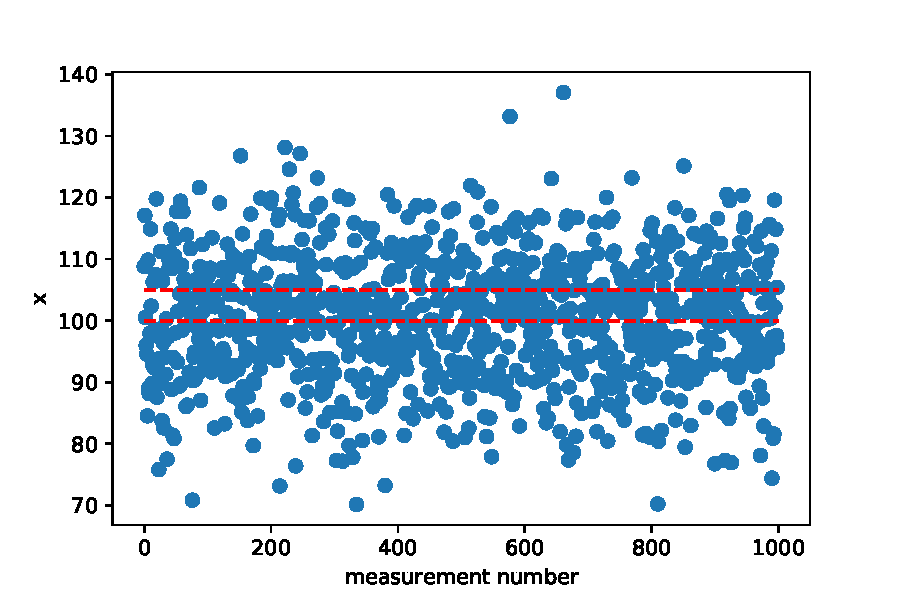
\includegraphics[width=0.45\textwidth]{figs/raw.pdf}} &
{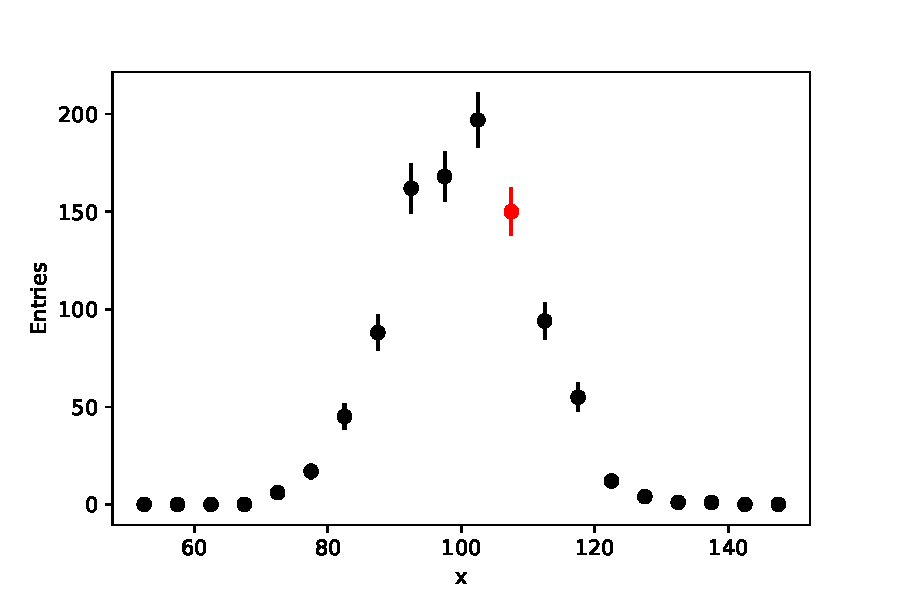
\includegraphics[width=0.45\textwidth]{figs/histeg.pdf}} \\
(a) & (b) \\
\end{tabular}
\end{center}
\caption{\label{fig:histeg} The 1000 measurements of variable $x$ in (a) are used to produce the histogram in (b).  The red data point in (b) is the count of the number of entries in range indicated by the red dashed lines in (a).}
\end{figure}

Suppose a particular variable $x$ is measured 1000 times.  One way to visualize the collected data is shown in Fig.~\ref{fig:histeg}a, which simply plots each measurement value above the measurement number (from 0 to 1000).  In this example, the number of measurements that occur within the range from $x=100$ to $x=105$ is 181.  This count is plotted as the red data point in Fig.~\ref{fig:histeg}b, 181 entries located above $x=102.5$, the center of the range.  If we repeat this exercise across a number or ranges, the resulting plot in Fig.~\ref{fig:histeg}b is called a histogram.  A histogram reports the number of entries that occur within each of a sequence of consecutive ranges of $x$-values.  Each range considered is called a histogram  bin, and the choice of which bins to use is at the discretion of the analyzer.

The content of each bin is a single number, a count. In
Section~\ref{sec:poissonmeanvar}, an appropriate estimate for typical
fluctuation of a count $N$ is shown to be $\sqrt{N}$.  It is customary
to indicate the size of these typical fluctuations with an ``error
bar'', a line through the data point at $N$ with length $\sqrt{N}$.
The error bars provide a visual cue to how much we expect that a
repeated identical measurement would vary with respect to the
presented data.

\begin{figure}[htbp]
\begin{center}
{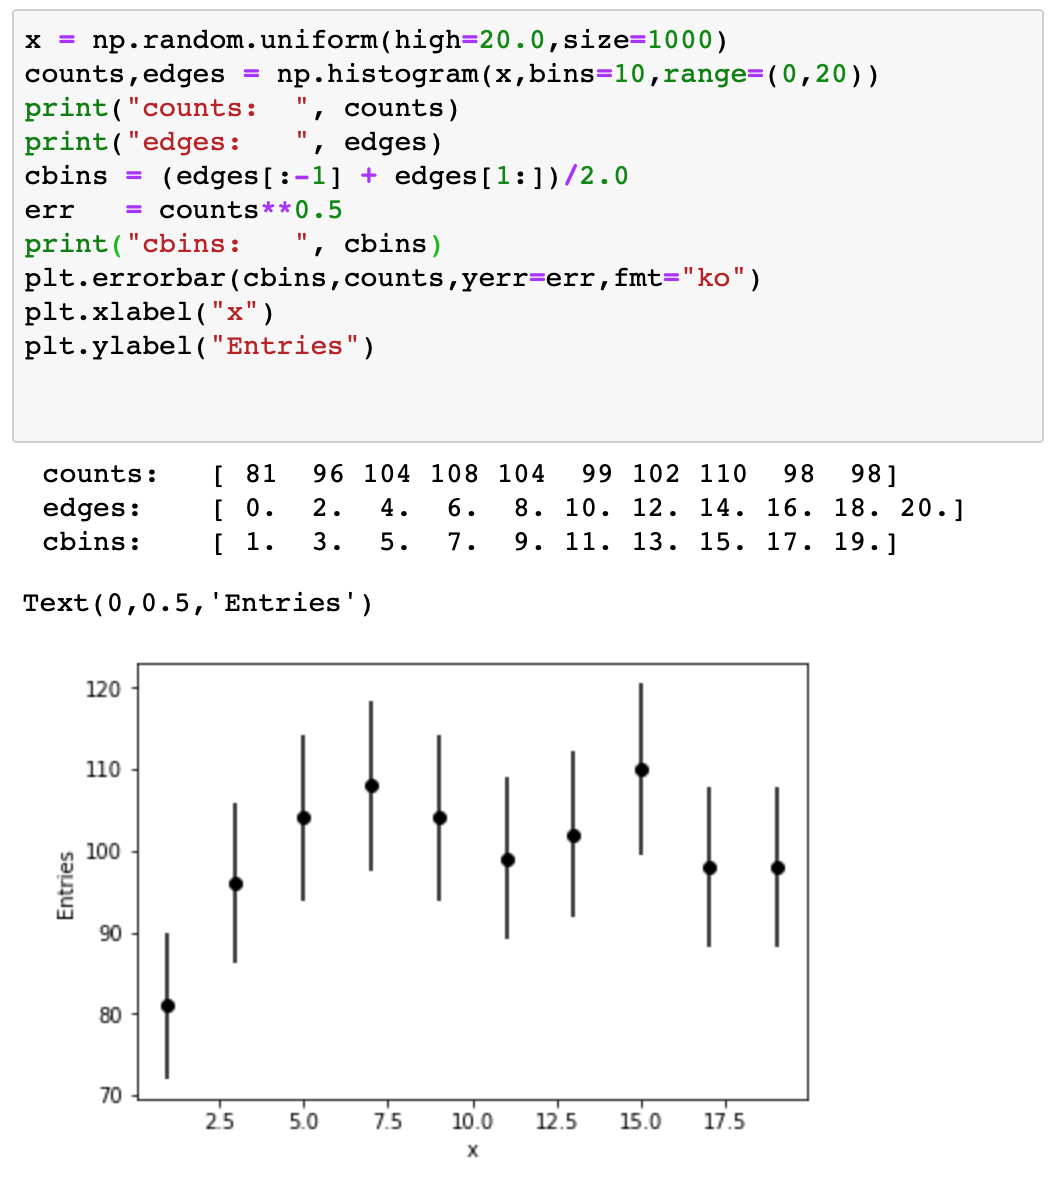
\includegraphics[width=0.85\textwidth]{figs/makehisteg.png}} 
\end{center}
\caption{\label{fig:makehisteg} Example producing a histogram in Scientific Python.}
\end{figure}

An example producing a histogram in Scientific Python is shown in Fig.~\ref{fig:makehisteg}.
The data to plot is simply a sequence of 1000 values randomly and uniformly chosen in the range $[0,20]$:
\begin{verbatim}
x = np.random.uniform(high=20.0,size=1000)
\end{verbatim}
To create a histogram from these 1000 values, we use the {\tt np.histogram} function:
\begin{verbatim}
counts,edges = np.histogram(x,bins=10,range=(0,20))
\end{verbatim}
where we have specified 10 bins, uniformly covering the range from 0 to 20.  The 
function returns to arrays, which we save as {\tt counts} and {\tt edges}.  The {\tt counts} array contains the bin contents, the count of the number of values in each bin: 
\begin{verbatim}
counts:   [ 92  82 123  96  85 106 105  99  99 113]
\end{verbatim}
The edges array contains the edges of the bins:
\begin{verbatim}
edges:    [ 0.  2.  4.  6.  8. 10. 12. 14. 16. 18. 20.]
\end{verbatim}
You'll notice that 10 consecutive bins have 11 edges.  For plotting continuous data, one choice is to plot the contents at the center of each bin:
\begin{verbatim}
cbins = (edges[:-1] + edges[1:])/2.0
\end{verbatim}
the two slices {\tt edges[:-1]} and {\tt edges[1:]} are all but the last and all but the first.  The average of the two is the center of each bin:
\begin{verbatim}
cbins:    [ 1.  3.  5.  7.  9. 11. 13. 15. 17. 19.]
\end{verbatim}
The error bar values are chosen as the square root of the bin values:
\begin{verbatim}
err   = counts**0.5
\end{verbatim}




The histogram is plotted using the {\tt plt.errorbar} function:
\begin{verbatim}
plt.errorbar(cbins,counts,yerr=err,fmt="ko")
\end{verbatim}
which plots the bin contents {\tt counts} at the bin center values {\tt cbins} using the square root error bars in the array {\tt err}, using the format {\tt "ko"} for black circles.

\section{Comparing a Histogram to a Probability Distribution Function}
\label{sec:comphist}


Our theoretical models often predict a PDF for some observable variable $x$.  As experimentalists, we are often therefore concerned with the question as to whether our collected data for an observable $x$ is consistent with the theoretical PDF.  A visual approach to answering this question is to plot the data in a histogram, and to draw the PDF as a curve normalized to the histogram.

To predict the number of events in a bin with edges $x_{\rm lower}$ and $x_{\rm upper}$, in principle we need to integrate the PDF and normalize to the number of experiments:
\begin{displaymath}
N_{\rm pred} = N_{\rm meas} \int^{x_{\rm upper}}_{x_{\rm lower}} p(x) \, dx
\end{displaymath}
In practice, we generally choose the bin sizes small enough that the PDF is approximately constant during the entire bin, and in this case, the prediction can be taken as:
\begin{displaymath}
N_{\rm pred} = N_{\rm meas} \; \Delta x \; p(x)
\end{displaymath}
where $\Delta x$ is the width of each bin.  This scale factor $N_{\rm meas} \; \Delta x$ allows us to compare a continuous function to data collected in discrete bins, as shown in Fig.~\ref{fig:histpdf}.

\begin{figure}[htbp]
\begin{center}
{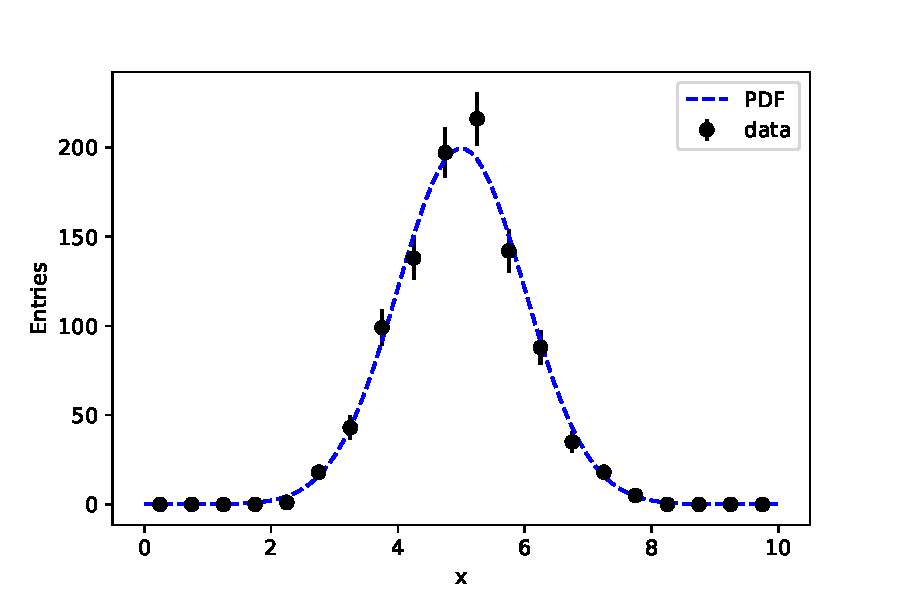
\includegraphics[width=0.65\textwidth]{figs/compare.pdf}}
\end{center}
\caption{\label{fig:histpdf} The Gaussian PDF scaled to compare to data from a Gaussian distribution.
In this case, there are 1000 total entries in the histogram and the bin size is 0.5, for a scale factor of 500.
}
\end{figure}



\newpage
\section{Homework Exercises for Distributions}

\noindent
{\bf Problem 1:} Show that the Binomial distribution, $P(m)$, in Equation~\ref{eqn:binom} is properly normalized:
\begin{displaymath}
\sum_{m=0}^n P(m) = 1
\end{displaymath}
as a consequence of the Binomial Theorem (Equation~\ref{eqn:binomt}).

\vskip 1cm
\noindent
{\bf Problem 2:} Show that Equation~\ref{eqn:varhw} is correct.

\vskip 1cm
\noindent
{\bf Problem 3:} Show that the Poisson distribution, $P(m)$, in Equation~\ref{eqn:poisson} is properly normalized:
\begin{displaymath}
\sum_{m \geq 0} P(m) = 1.
\end{displaymath}
Hint: recall the Taylor series expansion for $e^\lambda$.

\vskip 1cm
\noindent
{\bf Problem 4:} Show that the Gaussian distribution, $P(x)$, in Equation~\ref{eqn:gaussian} is properly normalized:
\begin{displaymath}
\int_{-\infty}^{\infty} P(x) dx = 1.
\end{displaymath}

\vskip 1cm
\noindent
{\bf Problem 5:} Show that the mean of the Gaussian distribution has been correctly identified in Equation~\ref{eqn:gaussian}.  That is, show explicitly that:
\begin{displaymath}
\int_{-\infty}^{\infty} x P(x) dx = \mu 
\end{displaymath}

\vskip 1cm
\noindent
{\bf Problem 6:} Show that the variance of the Gaussian distribution has been correctly identified in Equation~\ref{eqn:gaussian}.  That is, show explicitly that:
\begin{displaymath}
\int_{-\infty}^{\infty} x^2 P(x) dx = \sigma^2 
\end{displaymath}
when we take $\lambda=0$ (which is equivalent to simply changing variables $y=x-\lambda$.)

\vskip 1cm
\noindent
{\bf Problem 7:} Consider a special probability function with the following properties: (A) it is defined for outcomes 0,1,2,3, and 4, (B) it has two modes at outcomes 0 and 4, (C) it has three medians at outcomes 1,2, and 3.  Sketch the probability distribution and determine its mean. 

\noindent
{\bf Problem 9:} Suppose that two counting experiments $a$ and $b$ have outcomes that are well described by the Poisson distribution with mean values $\lambda_a$ and $\lambda_b$ respectively.  Now consider the counting
experiment $a+b$ that results from simply adding the counts from both experiments $a$ and $b$.  Show that that the variance of this sum is given by:
\begin{displaymath}
\sigma^2(a+b) = \sigma^2_a + \sigma^2_b
\end{displaymath}
We'll show in the next chapter that, quite generally, uncertainties $\sigma$ add in quadrature.

\newpage

\end{document}

\chapter{Experimental Uncertainties}

\section{Reporting Experimental Uncertainties}

\begin{figure}[htbp]
\begin{center}
{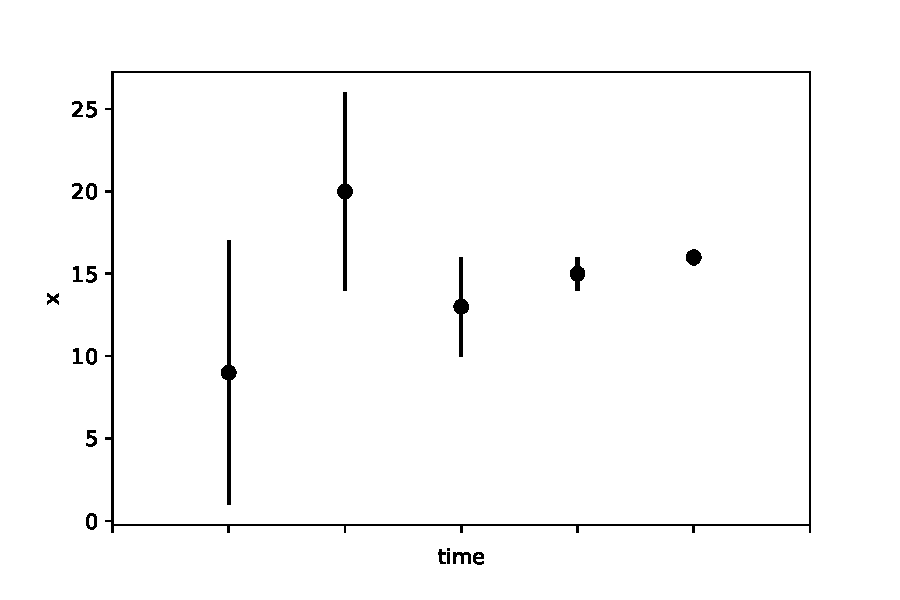
\includegraphics[width=0.45\textwidth]{figs/measuretime.pdf}}
\end{center}
\caption{\label{fig:measuretime}  The evolution of a measurement of a quantity $x$ over time.}
\end{figure}

A scientific measurement is meaningless without an associated uncertainty.   For instance, we might report a measured distance as:
\begin{displaymath}
x = 1.2 \pm 0.3~\rm m
\end{displaymath}
and a time as:
\begin{displaymath}
t = 4.76 \pm 0.13~\rm \mu s.
\end{displaymath}
When reporting a number with an associated uncertainty, we round both the value and the uncertainty to one significant digit in the uncertainty, so:
\begin{displaymath}
x = 1.245 \pm 0.313~{\rm m} \to x = 1.2 \pm 0.3~{\rm m} 
\end{displaymath}
If the first nonzero digit in the uncertainty is a zero or one, we keep two digits instead:
\begin{displaymath}
x = 1.245 \pm 0.113~{\rm m} \to x = 1.25 \pm 0.11~{\rm m}.
\end{displaymath}
We'll define this uncertainty quite precisely, but let's start with a
conceptual definition.  Each particular measurement of a quantity $x$
makes a claim about where the true value of $x$ is most likely to lie.
If we assume that measurements improve with time and better reproduce
the true value, we expect a series of measurements to proceed like in
Fig.~\ref{fig:measuretime}, with future measurements shown to be
consistent with the uncertainties reported by previous experiments.

\begin{figure}[htbp]
\begin{center}
{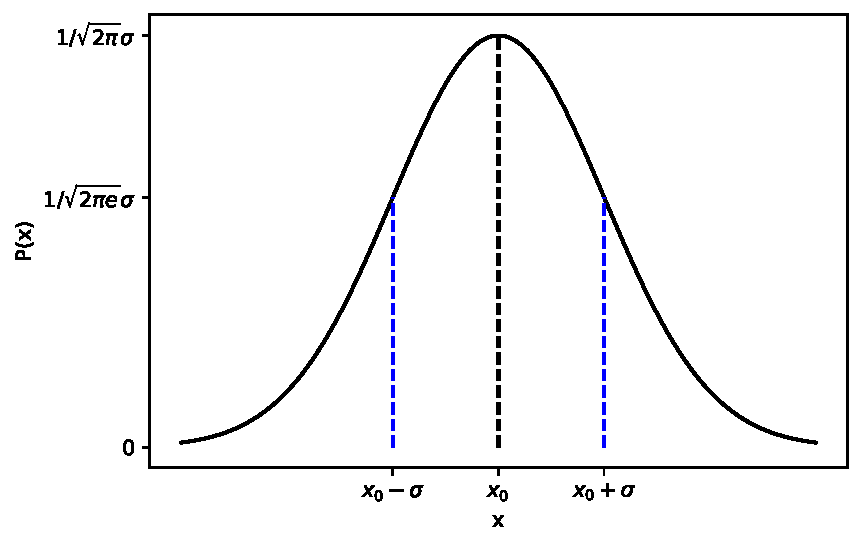
\includegraphics[width=0.45\textwidth]{figs/stdunc.pdf}}
\end{center}
\caption{\label{fig:stdunc}  The interpretation of experimental uncertainties as the parameters of a Gaussian distribution for the true value.}
\end{figure}

We can therefore think of a measurement and it's uncertainty as
describing a PDF for the outcome of experiments in the distant future
with uncertainties so small as to effectively measure the true value
of the quantity.  Because most measured quantities have many
independent sources of uncertainties, the Central Limit Theorem
implies that the true value of the measured quantity is best described
by a Gaussian Distribution.  We define the measured value $x$ as the
mean of this distribution, and the uncertainty as the $\sigma$ of the
Gaussian.

\section{The Error Function}

Suppose we measure the speed of light in vacuum to be:
\begin{displaymath}
3.3 \pm 0.2 \times 10^8~{\rm m}/{\rm s}^2
\end{displaymath}
How consistent is this with the generally accepted value:
\begin{displaymath}
3.0 \times 10^8~{\rm m}/{\rm s}^2
\end{displaymath}
where we have omitted the uncertainty here because it is much smaller than our uncertainty!   The interpretation of the uncertainty as the $\sigma$ of a Gaussian distribution allows us to give quite precise answers.  To begin we might say that it is consistent within:
\begin{displaymath}
\frac{3.3 - 3.0}{0.2} = 1.5 \; \sigma.
\end{displaymath}
but we can also ask, what is the probability enclosed in $1.5 \sigma$.  To  answer this question, we use the error function:
\begin{displaymath}
{\rm erf}(x) = \frac{1}{\sqrt{\pi}} \int^x_{-x} \exp\left(-t^2 \right) dt
\end{displaymath}
which is simply the integral from $-x$ to $x$ of a Gaussian with $\sigma = 1/\sqrt{2}$.  So if we want to calculate the probability contained in $n~\rm sigma$ we would calculate:
\begin{displaymath}
 {\rm erf}(n \cdot \frac{1}{\sqrt{2}})
\end{displaymath}
which is tabulated in Table~\ref{tbl:erf}.\\

\begin{table}[thb]
\begin{center}
\begin{tabular}{lll}
interval & error function & integrated probability \\ 
\hline
$\pm1 \sigma$ & ${\rm erf}\left( \frac{1}{\sqrt{2}} \right)$ & 68.3\% \\
$\pm2 \sigma$ & ${\rm erf}\left( \frac{2}{\sqrt{2}} \right)$ & 95.4\% \\
$\pm3 \sigma$ & ${\rm erf}\left( \frac{3}{\sqrt{2}} \right)$ & 99.7\% \\
$\pm4 \sigma$ & ${\rm erf}\left( \frac{4}{\sqrt{2}} \right)$ & 99.993\% \\
$\pm5 \sigma$ & ${\rm erf}\left( \frac{5}{\sqrt{2}} \right)$ & 99.99994\% \\ 
\end{tabular}
\caption{\label{tbl:erf} The integrated probability for a Gaussian distribution within the stated bounds.} 
\end{center}
\end{table}

In practice, scientist often speak in units of $\sigma$.  Measure
values that differs from a prediction by one or even two $\sigma$ are
generally considered to be consistent, because nearly $5\%$ of our
measurements will be off by two $\sigma$ or more.  At three sigma,
which occurs with a probabilty of $0.3\%$ things are starting to get
interesting: either someone has likely made a mistake (the theorist or
the experimentalist) or something new and exciting is happening, or
both.  In my field of particle physics, we consider three $\sigma$ to
constitute initial evidence, but hold off on claiming discovery of a
new particle until five $\sigma$.  This is because if you collect lots
of data and do lots of different analyses, it starts to become likely that
you will encounter occassional three $\sigma$ statistical fluctuations.

\section{Mean and Variance of a Sum}

So far we've been calculating expectation values of functions of one random variable: 
\begin{displaymath}
\braket{f(x)} = \int f(x) \; P(x) \; dx
\end{displaymath}
but this easily generalizes to two or more random variables:
\begin{displaymath}
\braket{f(x,y)} = \int \int f(x,y) \; P(x,y) dx \, dy 
\end{displaymath}
If the random variables are independent, then we have $P(x,y) = P(x) \, P(y)$ and so
\begin{displaymath}
\braket{f(x,y)} = \int f(x,y) \; P(x) \, P(y) \; dx \, dy
\end{displaymath}
And also we have
\begin{eqnarray*}
\braket{f(x)+g(y)} &=& \int \int dx \, dy \; P(x) \, P(y) \;\; (f(x) + g(y)) \\
&=& \left(\int P(y) \; dy \right) \cdot \left( \int P(x) \; f(x) \; dx  \right) 
+ \left(\int P(x) \; dx \right) \cdot \left( \int P(y) \; f(y) \; dy  \right)\\
&=& 1 \cdot \int P(x) \; f(x) \; dx  + 1 \; \cdot \int P(y) \; f(y) \; dy \\
\end{eqnarray*}
which we can write much more simply as:
\begin{displaymath}
\braket{f(x)+g(y)} = \braket{f(x)}+\braket{g(y)}
\end{displaymath}
revealing the power of the expectation value notation for tackling independent random variables.  In the homework you will show that similarly:
\begin{equation}
\braket{f(x) \cdot g(y)} = \braket{f(x)} \cdot \braket{g(y)} \label{eqn:expprod}
\end{equation}
We can therefore conclude that the mean of a sum of two random variables:
\begin{displaymath}
\braket{x + y} = \braket{x} + \braket{y} 
\end{displaymath}
is just the sum of the mean.  

For simplicity let's assume that $\braket{x} = \braket{y} = 0$, and so:
\begin{eqnarray*}
\braket{(x + y)^2} &=& \braket{x^2 + 2xy + y^2} \\
&=& \braket{x^2} + 2\braket{xy} + \braket{y^2} \\
&=& \braket{x^2} + 2\braket{x}\braket{y} + \braket{y^2} \\
&=& \braket{x^2} + \braket{y^2} \\
\end{eqnarray*}
from which it follows that:
\begin{eqnarray*}
\sigma^2(x+y) &=& \braket{(x+y)^2} - \left( \braket{x+y} \right) ^2\\
&=& \braket{(x+y)^2}\\
&=& \braket{x^2} + \braket{y^2} \\
&=& \sigma^2_x + \sigma^2_y\\
\end{eqnarray*}
In the exercises you will show that even if $\braket{x}$ and $\braket{y}$ are non-zero, we still obtain:
\begin{displaymath}
\sigma^2(x+y) = \sigma^2_x + \sigma^2_y
\end{displaymath}
that is, the uncertainties in a sum add in quadrature.

\section{Independent Uncertainties Add in Quadrature}

In the previous section, we discussed that the variance of the sum of two random variables drawn from any distribution is just the sum of their variances:
\begin{displaymath}
\sigma^2(x+y) = \sigma^2_x + \sigma^2_y
\end{displaymath}
This is a quite general result.  In the context of experimental uncertainties, we consider experimental measurements to be drawn from a Gaussian distribution and the square-root of the variance ($\sigma$) is called the uncertainty.

If we calculate the sum $s$ of two independent measurements $x$ and $y$ with uncertainties $\sigma_x$ and $\sigma_y$, it's clear that the variance of the sum will be simply $\sigma^2_x + \sigma^2_y$.  If the resulting distribution of $x+y$ is a Gaussian distribution, as seems probable due to the Central Limit Theorem, then the uncertainties simply add in quadrature:
\begin{displaymath}
\sigma_{x+y} = \sqrt{\sigma^2_x + \sigma^2_y}.
\end{displaymath}

Let's show explicitly that this is the case.  If we wish to know the probability that two random variables $x$ and $y$ add to some particular value $u = x + y$, we simply integrate the total probability of $x$ and $y$ subject to the requirement $u = x + y$:
\begin{eqnarray*}
P(u) &=& \int dx \int dy \; P_x(x) \, P_y(y) \, \delta\left(u-(x+y)\right) \\
        &=& \int dx \; P_x(x) \, P_y(u-x)
\end{eqnarray*}
If we make the (very often valid) assumption that $x$ and $y$ are Gaussian distributed, and, for simplicity, assume that the mean values are zero (or simply change coordinates), so that we have:
\begin{eqnarray*}
P_x(x) &=& \frac{1}{\sqrt{2\pi} a} \exp\left( -\frac{x^2}{2a^2} \right) \\
P_y(y) &=& \frac{1}{\sqrt{2\pi} a} \exp\left( -\frac{y^2}{2b^2} \right) 
\end{eqnarray*}
And so the mean value probability distribution function for $u$ is now:
\begin{eqnarray*}
P(u) &=& \frac{1}{2\pi a b} \int dx \; \exp\left( -\frac{x^2}{2a^2}\right) \exp\left( -\frac{(u-x)^2}{2b^2}\right) \\
&=& \frac{1}{2\pi a b} \int dx \; \exp \left( -\frac{a^2+b^2}{2a^2b^2} \, \left\{ x^2 - \frac{2a^2}{a^2+b^2}ux + \frac{a^2}{a^2+b^2}u^2\right\}_1 \right) 
\end{eqnarray*}
We deal with the term in brackets ($\{\}_1$) by completing the square.  Simply note that
\begin{equation}
\left(x-\frac{a^2}{a^2+b^2}u\right)^2 = x^2-\frac{2a^2}{a^2+b^2}ux + \frac{a^4}{(a^2+b^2)^2}u^2
\end{equation}
reproduces the first and second terms, so we can replace:
\begin{equation}
x^2-\frac{2a^2}{a^2+b^2}ux  = \left(x-\frac{a^2}{a^2+b^2}u\right)^2 -  \frac{a^4}{(a^2+b^2)^2}u^2
\end{equation}
to obtain:
\begin{eqnarray*}
\{\}_1 &=& \left(x-\frac{a^2}{a^2+b^2}u\right)^2 -  \frac{a^4}{(a^2+b^2)^2}u^2 + \frac{a^2}{a^2+b^2}u^2\\
&=& \left(x-\frac{a^2}{a^2+b^2}u\right)^2 + \frac{a^2b^2}{(a^2+b^2)^2}u^2\\
\end{eqnarray*}
and substituting back into the original expression we obtain:
\begin{eqnarray*}
P(u) &=& \frac{1}{2\pi a b} \left\{ \int_{-\infty}^{+\infty} dx \;  \exp \left( -\frac{a^2+b^2}{2a^2b^2} \, \left(x-\frac{a^2}{a^2+b^2}u\right)^2 \right) \right\}_2
\exp \left( -\frac{1}{2} \frac{u^2}{a^2+b^2} \right)
\end{eqnarray*}
making a substitution of variables ($u$ is constant during the integration):
\begin{equation*}
y = x-\frac{a^2}{a^2+b^2}u
\end{equation*}
the definite integral in brackets yields:
\begin{equation}
\{\}_2 = \sqrt(2 \pi) \frac{a b}{\sqrt{a^2+b^2}}
\end{equation}
and we have at last:
\begin{eqnarray*}
P(u) &=& \frac{1}{\sqrt{2\pi} \sqrt{a^2+b^2}}  \exp \left( -\frac{1}{2} \frac{u^2}{a^2+b^2} \right)
\end{eqnarray*}
which is a Gaussian distribution with variance:
\begin{eqnarray*}
\sigma^2 = a^2 + b^2,
\end{eqnarray*}
that is, uncertainties add in quadrature.

\section{Handling Constants}

When adding a known constant to a measured quantity:
\begin{equation*}
y = x + C
\end{equation*}
we can consider the constant to have uncertainty $\sigma=0$.  And therefore, from the addition in quadrature rule:
\begin{equation*}
\sigma_y = \sigma_x
\end{equation*}

If we multiply a measured quantity by a known constant 
\begin{equation*}
y = k x 
\end{equation*}
we consider that:
\begin{displaymath}
dx \frac{1}{\sqrt{2\pi} \sigma} \exp\left(-\frac{(x-\mu)^2}{2\sigma^2}\right) = d(kx) \frac{1}{\sqrt{2\pi} k\sigma} \exp\left(-\frac{(kx-k\mu)^2}{2(k\sigma)^2}\right)
\end{displaymath}
and conclude that:
\begin{equation*}
\sigma_y = k \sigma_x
\end{equation*}

\section{Repeated Experiments}

Suppose that we have an apparatus which can measure a quantity $x$
with uncertainty $\sigma_x$, and that we repeat a series of $N$
measurements $x_1$, $x_2$, $x_3$, \ldots, $x_N$. Each $x_i$ is a
random variable drawn from a distribution with variance $\sigma_x$ and
mean $\mu$.

A useful quantity to calculate from our $N$ measurements is the sample mean:
\begin{displaymath}
  \bar{x} \equiv \frac{1}{N} \, \sum_{i=1}^{N} x_i = \frac{x_1 + x_2 + x_3 + \ldots + x_N}{N}
\end{displaymath}
Just as each of our individual measurements have mean value:
\begin{displaymath}
\braket{x_i} = \mu  
\end{displaymath}
the sample mean also has mean value:
\begin{displaymath}
  \braket{\bar{x}} = \frac{1}{N} \, \sum_{i=1}^{N} \braket{x_i}
= \frac{1}{N} \, \sum_{i=1}^{N} \mu = \mu
\end{displaymath}
The uncertainty on the sample mean can be calculated using the results of the previous sections which covered sums and constant scale factors:
\begin{eqnarray*}
  \sigma^2(\bar{x}) &=& \sigma^2\left( \frac{1}{N} \, \sum_{i=1}^{N} x_i \right) \\
  &=& \sum_{i=1}^{N} \left( \sigma \left( \frac{x_i}{N} \right) \right)^2 \\
  &=& \sum_{i=1}^{N} \left( \frac{\sigma_x}{N} \right)^2 \\ 
  &=& \frac{\sigma_x^2}{N} \\
 \sigma_{\bar{x}} &=& \frac{\sigma_x}{\sqrt{N}} \\
\end{eqnarray*}
This shows that the sample mean measures the same mean value $\mu$ but
with an uncertainty that is reduced by a factor $1/\sqrt{N}$.  More
generally, taking additional data reduces the uncertainty of a
measurement.  If you take gfour times as much data, you can expect the
uncertainties to be cut in half.

Statistics textbooks will often refer to $\mu$ as the {\em poplulation
  mean} and $\bar{x}$ as the {\em sample mean}, terminology that makes
good sense in the context of estimating properties of an entire
population using a smaller sample.  I've mostly avoided this
terminology because it doesn't make as much sense in the context of
measurement of most physics experiments where this is no finite
population to consider.  We are generally attempting to measuring
fundamental properties of the universe, not hair length in a
population of goats!  But you'll likely encounter this terminology in
the statostics literature.

\section{General Propagation of Uncertainties}

We are now ready to handle propagation of uncertainties for a general
function.  Suppose we measure $x = x_0 \pm \sigma_x$ and $y = y_0 \pm
\sigma_y$ and we wish to know the resulting uncertainty on the
calculated quantity $f(x,y)$.

Now we Taylor expand the function about the measured values $x_0$ and $y_0$:
\begin{equation*}
f(x,y) \sim f(x_0,y_0) + \left.\frac{\partial f}{\partial x}\right|_{x_0,y_0} (x-x_0) + \left.\frac{\partial f}{dy}\right|_{x_0,y_0} (y-y_0) 
\end{equation*}
which we can write as:
\begin{equation*}
f(x,y) \sim A + B x + C y 
\end{equation*}
where the constants are:
\begin{eqnarray*}
  A  &=& f(x_0,y_0) - B x_0 - C y_0\\
  B  &=& \left.\frac{\partial f}{\partial x}\right|_{x_0,y_0}\\
  C  &=& \left.\frac{\partial f}{dy}\right|_{x_0,y_0}\\
\end{eqnarray*}
We know how to propagate uncertainties in this case, which involves scaling, adding in quadrature, and adding a constant:
\begin{equation*}
\sigma_f^2 =   B^2 \sigma_x^2 + C^2 \sigma_y^2 
\end{equation*}
And plugging in the constants:
\begin{equation*}
\sigma^2_f = \left(\left.\frac{\partial f}{\partial x}\right|_{x_0 y_0} \right)^2 \sigma^2_x  + \left( \left.\frac{\partial f}{dy} \right|_{x_0 y_0} \right)^2 \sigma^2_y
\end{equation*}   
This is a plausible result.  As $x$ moves by a typical amount $\sigma_x$ from the value $x_0$, we expect $f$ to change by approximately:
\begin{equation*}
  \Delta f = \left.\frac{\partial f}{\partial x}\right|_{x_0 y_0} \sigma_x
\end{equation*}   
The result we obtain is this amount of variation added in quadrature with a similar variation due to variable $y$.

This result was obtained by the Taylor series approximation, and is
therefore only appropriate when the uncertainties are small enough
that the function $f$ is not changing dramatically as $x$ and $y$ vary
by $\sigma_x$ and $\sigma_y$.  This is usually the case for a well
designed experiment.  A poorly designed experiment that determines a
quantity $f$ which is varying dramatically, from poorly measured
quantities, would likley benefit from a redesign, for instance by
measuring the dramatically varying quantity $f$ more directly!  A
typical case where this approximation is problematic is when
calculating recipocals of quantities which are within a few sigma of
zero.

\section{Systematic Uncertainties}

If by repeating an experiment $N$ times we can reduce the statistical
uncertainty by a factor of $\sqrt{N}$, it might seem that we can reach
any desired level of experimental uncertainty simply by repeating an
experiment many times.  Unfortunately, statistical uncertainty is just
one component of experimental uncertainty.  There is also systematic
uncertainty.

Our derivation of the Binomial, Poisson, and Gaussian distributions
all shared a common assumption: that each outcome is independent of
previous outcomes.  But real measurements are also biased from the
correct value by a {\bf constant} and unknown amount.  We describe the
expected size of this bias as an additional uncertainty called the
systematic uncertainty.  Since the bias away from the true value is
constant, and not subject to statistical fluctuations, repeating an
experiment does nothing to reduce systematic uncertainties.  The only
way to reduce systematic uncertainties is to design a better
experiment.  Generally in the early stages, experiments are
statistically limited, and taking more data helps reduce the overall
uncertainty.  But at a later stage, the experiment becomes
systematically limited.  More data does not help unless the apparatus
is improved.  Often, in complicated experiments, increased statistics
also gives the experimenter a better handle on the systematic
uncertainties, allowing for improvements to both the statistical and
systematic uncertainties.

The treatment of systematic uncertainties is one of the greatest challenges that an experimenter faces.  
Often scientific results report a measurement with both the statistical and a systematic uncertainty, e.g.:
\begin{displaymath}
 x = 1.21 \pm 0.03 ({\rm stat}) \pm 0.05 ({\rm syst})
\end{displaymath}
Systematic uncertainties and statistical uncertainties are considered to be independent, so the total experimental uncertainty is their sum in quadrature:
\begin{displaymath}
\sigma_{\rm total} = \sqrt{\sigma^2_{\rm syst} + \sigma^2_{\rm stat}}.
\end{displaymath}

Often, systematic uncertainties are the result of something outside the experimenters direct control.  One common example is when a measurement depends on a measured value determined by another experiment.  For example, suppose you determine a position $x$ from your measurement of a time $t$ by the relation $x = v t$.  But you do not measure the velocity $v$ yourself and instead rely on a previous measurement of $v$ with total uncertainty $\sigma_v$.  In this case, by standard propagation of uncertainties, we find that:
\begin{displaymath}
\frac{\sigma_x}{x} = \frac{\sigma_v}{v}.
\end{displaymath}
So a $10\%$ uncertainty on the value $v$ would lead to a $10\%$ systematic uncertainty on our measured value $x$.

Another common source of systematic uncertainties is when a measured value depends on something outside the experimenters direct control.   These types of uncertainties are usually estimated by determining how much the uncontrolled quantity is likely to vary, and the effect this variation has on the measured value.  For example, suppose a measurement was sensitive to the amount of light that leaks into the apparatus, which is different depending on the weather and time of day.  In this case, you might estimate the systematic by comparing results of measurements made at noon to similar measurements made at midnight.

Apart from building a better experiment, the most common way to improve systematics is by calibration.  You could eliminate the systematic due to the velocity $v$ in the first example by measuring the relationship between $x$ and $t$ yourself.  In the light leakage example, you could record the time each measurement was made, and correct for the effect of light leakage.  

\section{Exercises for Uncertainties}


\noindent
{\bf Problem 1:}  Suppose you measure an RMS voltage as $V = 43.2145~\rm mV$ and you calculate the uncertainty on this measurement to be $0.471~\rm mV$.  How should you report this measurement?  How about if the uncertainty were $1.07~\rm mV$? \\ \vskip 0.25cm

\noindent
{\bf Problem 2:}  Show that Equation~\ref{eqn:expprod} is valid. \\ \vskip 0.25cm

\noindent
{\bf Problem 3:}  Show that for independent random variables $x$ and $y$:
\begin{displaymath}
\braket{(x+y)^2} - \braket{x+y}^2 = \braket{x^2} - \braket{x}^2 + \braket{y^2} - \braket{y}^2.
\end{displaymath}
What does this imply about the uncertainty on the sum of two variables, assuming all of the PDFs are Gaussian? \\ \vskip 0.25cm

\noindent
{\bf Problem 4:}  For a measurement $x_0 \pm \sigma$ we define the fractional uncertainty as $\sigma/x_0$.  Use the general formula for propagating uncertainties to show that for products and ratios, the {\em fractional} uncertainties add in quadrature.  \\ \vskip 0.25cm

\noindent
{\bf Problem 5:}  Suppose you measure the system gain (i.e. the increase in output voltage for each electron) for your new ionization chamber to be $12~\rm mV$ per collected electron.  Suppose you measure a pulse with a height of $6.2~\rm V$.  First estimate the uncertainty on this measured value due to statistical fluctuations from the number of electrons.   You can neglect any uncertainties on the system gain measurement and the voltage reading itself as these are very small compared to the uncertainty due to electron statistics.  Next, suppose your pre-amplifier adds about $300~\rm mV$ of noise to this measurement.  What is the total uncertainty for this measurement? \\ \vskip 0.25cm

\noindent
{\bf Problem 6:}  The rare decay of the Higgs boson ($m \sim125~\rm GeV$ in units where $c=1$) into pairs of photons played a crucial role in its discovery at the Large Hadron Collider.  The invariant mass of a particle that decays into two massless particles $p_1$ and $p_2$ can be calculated from:
\begin{displaymath}
m = \sqrt{2  p_1 p_2 (1 - \cos\theta)}
\end{displaymath}
Suppose you were sitting in the control and saw a nice looking two photon event with 
$p_1=53 \pm 2~\rm GeV$, $p_2=75 \pm 3~\rm GeV$ and $\theta = 2.8 \pm 0.1$.   Calculate the invariant mass of these two photons (answer in GeV) and the uncertainty. \\ \vskip 0.25cm

\noindent
{\bf Problem 7:}  A perennial problem with drawing data in histograms is what to do about bins that have zero events in them.  Those crazy people that insist that data has no statistical uncertainty (only predictions have statistical uncertainty!) laugh maniacally when we struggle with what to do in these bins.  This is where our highly useful fiction that data has an associated uncertainty manifestly falls apart! 

The crazy people argue like this: the Poisson distribution has one parameter $\lambda$ which is both the mean and the variance.  We expect to see $\lambda$ events on average with fluctuations of about $\sigma = \sqrt{\lambda}$, leading to some observed value $n$.  When we plot uncertainties of $\sqrt{n}$ we are plotting the wrong uncertainty, which should be $\sqrt{\lambda}$.  Calculate how much these two estimates vary for a typical one sigma fluctuation, up and down, for $\lambda=10$ and $\lambda=100$.  Do the crazy people have a point? \\ \vskip 0.25cm

\noindent
{\bf Problem 8:}  In particle physics, we always need to understand the efficiency of our detectors.  For instance, if $n$ muons are produced by collisions, we'd like to know how many are actually recorded successfully by our muon detectors.  If we measure $m$ muons that are actually detected, we know that our efficiency is $\epsilon = m/n$.  No problem here!

You will often see young particle physicists (and occasionally old!) run into problems estimating the uncertainty of this estimate.  They reason like this:  $n$ is just a constant, with no uncertainty.  I could pick to study exactly 1000 events, for instance.  The only number which I actually measure is $m$, and that should fluctuate by $\sigma_m = \sqrt{m}$.  So my uncertainty on the efficiency is just $\sigma_\epsilon = \sigma_m/n = \sqrt{m}/n$.  Problems arise because we often build good detectors with high efficiency.  So consider, for instance $n=100$ and $m=95$.  This leads to a measurement of the efficiency as $0.95 \pm 0.10$ which seems to include the impossible value $\epsilon = 1.05$.

One way out of this embarrassment is to realize that this problem is more appropriate for the binomial distribution which has two parameters, the number of trials $n$ and the success rate $\epsilon$ which is precisely the efficiency we are attempting to measure, and for which we all agree our best estimate is $\epsilon = m/n$.  Unlike our incorrect assumption that $\sigma_m = \sqrt{m}$, for the Binomial distribution
$\sigma_m = \sqrt{n \epsilon (1 - \epsilon))}$.  Calculate the resulting uncertainty on the efficiency 
$\epsilon$ and check that there is no longer a problem for $n=100$ and $m=95$.

There's another way to solve this problem, and that is to realize that $m$ and $n$ are not independent variables, because $m > n$ is impossible.  If we instead think of this in terms of the number of events $p$ that pass, and the number of events $f$ that fail, these variable are independent.  Calculate the uncertainty on the efficiency: 
\begin{displaymath}
\epsilon = \frac{p}{p+f}
\end{displaymath}
using standard propagation of uncertainties and the fact that $\sigma_p = \sqrt{p}$ and $\sigma_f = \sqrt{f}$.  You should be able to reproduce the same answer as above. \\ \vskip 0.25cm




%\chapter{Challenges (Not Assigned)}
%
%\noindent
%{\bf Problem 1:} Prove by induction the formula for the binomial coefficients in (Equation~\ref{eqn:binomc}).


\chapter{Statistical Analysis}

\section{Likelihood and $\chi^2$}

Suppose we make a series of measurements:
\begin{displaymath}
\{x_1 \pm \sigma_1, x_2 \pm \sigma_2, \ldots, x_n \pm \sigma_n \} \equiv x_i \pm \sigma_i
\end{displaymath}
and we would like to quantify how likely this outcome is to have occurred as the result of a corresponding theoretical prediction for each measurement:
\begin{displaymath}
\{X_1, X_2, \ldots, X_n \} \equiv X_i
\end{displaymath}
Assuming the uncertainties on each $x$ are Gaussian, the probability of one measurement is:
\begin{displaymath}
P_i = \frac{1}{\sqrt{2 \pi} \sigma_i}  \exp\left( - \frac{(X_i-x_i)^2}{2\sigma_i^2}\right)
\end{displaymath}
And the probability for the complete set of measurements, called the Likelihood, is the product of these probabilities for each measurement:
\begin{displaymath}
{\cal L} = \prod_i P_i = \prod_i \frac{1}{\sqrt{2 \pi} \sigma_i}  \exp\left( - \frac{(X_i-x_i)^2}{2\sigma_i^2}\right)
\end{displaymath}
Now being physicists, we hate products and prefer sums, so we apply a logarithm , and there is an annoying factor of $\frac{1}{2}$ in the exponential, so we multiple by 2.  We'd also like to construct a quantity that tells us about how far apart a prediction is from our measurement, and so we multiply by $-1$, to obtain:
\begin{equation}
-2 \log {\cal L} = \sum_i \frac{(X_i-x_i)^2}{\sigma_i^2} + 2 \log(\sqrt{2\pi}\sigma_i)
\end{equation}
Assuming the experimental uncertainties, $\sigma_i$, are known, the second term is simply a constant of the experiment setup.  The first term is what we call the $\chi^2$ metric:
\begin{equation}
\chi^2 \equiv \sum_i \frac{(X_i-x_i)^2}{\sigma_i^2} 
\end{equation}
A small value of $\chi^2$ means that the result is close to the theoretical prediction and a large value means that the result is unlikely to have occurred as a result of the prediction.  If the uncertainties and prediction are all correct, we would expect each $x_i$ to differ from the prediction $X_i$ by about $\sigma_i$.  So in this case we would expect:
\begin{equation}
\chi^2 = \sum_i \frac{(X_i-x_i)^2}{\sigma_i^2} \sim \sum_i 1 = N
\end{equation}
This assumes that the prediction $X_i$ is simply given to us.  We'll revisit this assumption when we discuss degrees of freedom.

\section{Maximal Likelihood Method}

Often, we are interested to know which particular parameters of a model maximize the likelihood
of the data we have collected.  For instance, suppose we made $N$ measurements:
\begin{displaymath}
\left\{ x_1 \pm \sigma, x_2 \pm \sigma, ..., x_N \pm \sigma \right\}
\end{displaymath}
of the same quantity, and we would like to find out which single value $X$ is most consistent with these $n$ measurements.  Our $\chi^2$ for this simple model is then:
\begin{displaymath}
\chi^2 = \sum_i \frac{(X - x_i)^2}{\sigma^2}.
\end{displaymath}
We can find the particular value of $X$ that maximizes the likelihood by finding the value that minimizes the $\chi^2$, because $\chi^2 \sim - 2 \log \mathcal{L}$.  We find the minimum from the condition:
\begin{displaymath}
\frac{d\chi^2}{\partial x} = 0,
\end{displaymath}
which amounts to:
\begin{eqnarray}
0 &=& 2 \sum_i \frac{(X - x_i)}{\sigma^2} \nonumber \\
0 &=& \left( X \sum_i \right)- \left( \sum_i x_i \right) \nonumber \\
X &=& \frac{1}{N} \sum_i x_i \label{eqn:mean}
\end{eqnarray}
which of course is just the mean of the measurements, as expected.

The $\chi^2$ formalism is quite general.  Suppose at each position $x_i$ we make a measurement $y_i$ which has a corresponding theoretical prediction $f(x_i; a, b)$ where $a$ and $b$ are parameters of the theory.  In this case, the $\chi^2$ is given:
\begin{displaymath}
\chi^2 = \sum_i \frac{(f(x_i;a,b) - y_i)^2}{\sigma_i^2}
\end{displaymath}
and to determine the best fit values for $a$ and $b$ we would require:
\begin{eqnarray*}
\frac{\partial \chi^2}{\partial a} &=& 0 \\
\frac{\partial \chi^2}{\partial b} &=& 0 
\end{eqnarray*}
We can accommodate any number of theory parameters in this fashion.  And the interpretations of $x$ and $y$ are endless.  We can imagine taking measurements of the voltage at particular times, measuring the electric field strength at particular radii, the number of cars produced in a factory each month, and so on.

\section{Interpretation of $\Delta \chi^2$}

\begin{figure}[htbp]
\begin{center}
{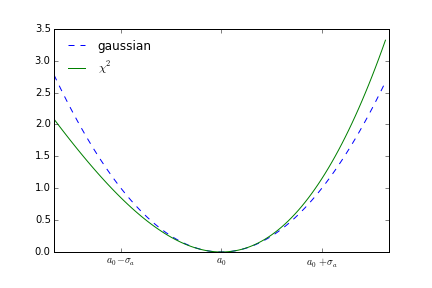
\includegraphics[width=0.75\textwidth]{figs/chisq.png}}
\end{center}
\caption{\label{fig:chisq} Approximation of $\chi^2$ near minimum.}
%x = np.arange(0,10,0.1)
%y = (x - 5)**2/3**2
%z = y + 0.05*(x - 5)**3/3**2 
%plt.plot(x,y,"--",label="gaussian")
%plt.plot(x,z,"-",label="$\chi^2$")
%plt.legend(loc=2,frameon=False)
%plt.xticks([2,5,8],["$a_0 - \sigma_a$", "$a_0$", "$a_0 + \sigma_a$"])
%plt.savefig("chisq.png")
\end{figure}

Suppose at particular points $\{x_i\}$ we have made measurements $\{y_i \pm \sigma_i\}$ with corresponding theoretical predictions $f(x_i, a)$.  Using the $\chi^2$ formalism we can determine the best fit value $a_0$ for the parameter $a$.  But this is of very little use unless we can also determine the corresponding uncertainty $\sigma_a$ associated with the best fit value $a_0$.  

One approach is to simply apply propagation of uncertainties to the formula determined by minimizing the $\chi^2$, for instance, Equation~\ref{eqn:mean}.  But this approach can be tedious or even unusable in cases where the $\chi^2$ is minimized numerically and no closed form solution is available.   It is well worthwhile, therefore, to consider an alternative approach, that determines these uncertainties directly from the Likelihood and its corresponding $\chi^2$ distribution.

Consider the Likelihood associated with this series of measurements:
\begin{displaymath}
\mathcal{L}(a) = \prod_i \frac{1}{\sqrt{2\pi} \sigma_i} \exp\left(-\frac{1}{2} \frac{(f(x_i,a)-y_i)^2}{\sigma_i^2}\right)
\end{displaymath}
This complicated function in the end is just the PDF for the true value of the parameter $a$, as determined by our data.  We are well justified, therefore, to assume this PDF is equivalently a simple Gaussian distribution: 
\begin{displaymath}
\mathcal{L}(a) =  \frac{1}{\sqrt{2\pi} \sigma_a} \exp\left(-\frac{(a-a_0)^2}{2\sigma_a^2}\right)
\end{displaymath}
explicitly in terms of the best fit value $a_0$ and the uncertainty $\sigma_a$.  The $\chi^2$ is then simply:
\begin{equation} \label{eqn:chisqa}
\chi^2(a; a_0, \sigma_a) = \frac{(a-a_0)^2}{\sigma_a^2}
\end{equation}
We see that:
\begin{displaymath}
\frac{d\chi^2}{da} = \frac{2 (a-a_0)}{\sigma_a^2} = 0
\end{displaymath}
when $a=a_0$ exactly as expected.  We also see that:
\begin{displaymath}
\frac{d^2\chi^2}{da^2} = \frac{2}{\sigma_a^2}
\end{displaymath}

As shown in Fig.~\ref{fig:chisq} the $\chi^2$ for a Guassian likelihood is a parabola, and so the second derivative {\em evaluated anywhere} yields a term containing the uncertainty $\sigma_a$.  However, the region near the minimum of any $\chi^2$ can distribution can be approximated as a parabola about the minimum, and so for a general $\chi^2$ distribution, we have:
\begin{equation} \label{eqn:chisqunc}
\sigma_a^2  = \frac{2}{\left. \frac{d^2\chi^2}{da^2} \right|_{a_0}}
\end{equation}
The uncertainty on any parameter can be estimated from the curvature of the $\chi^2$ at the minimum.
Another approach, sometimes used in numerical calculations, is to note that $\chi^2$ changes by a factor of one when you move a distance $\sigma_a$ from the minimum.

\section{Uncertainty on the Mean}

Earlier we used the $\chi^2$ formalism to show that the best fit constant value describing a set of repeated measurements of the same quantity:
\begin{displaymath}
\left\{ x_1 \pm \sigma, x_2 \pm \sigma, ..., x_N \pm \sigma \right\} \equiv x_i \pm \sigma_i
\end{displaymath}
is, not surprisingly, the mean value of the data:
\begin{displaymath}
X_0 = \frac{1}{N} \sum_i x_i \label{eqn:mean}.
\end{displaymath}
We are now in a position to determine the uncertainty on this mean value, by first taking the second derivative of the $\chi^2$ function:
\begin{eqnarray*}
\chi^2 &=& \sum_i \frac{(X-x_i)^2}{\sigma^2} \\
\frac{d\chi^2}{dX} &=& \sum_i \frac{2\,(X-x_i)}{\sigma^2}\\
\frac{d^2\chi^2}{dX^2} &=& \sum_i \frac{2}{\sigma^2}\\
&=& \frac{2 N}{\sigma^2}\\
\end{eqnarray*}
From which we conclude that the uncertainty on the mean is given by:
\begin{displaymath}
\sigma^2_X = \frac{2}{\left. \frac{d^2\chi^2}{dX^2} \right|_{X_0}} = \sigma^2 / N
\end{displaymath}
a result we obtained before by simply propagating uncertainties.

\section{Weighted Mean}

Suppose we make a series of measurements of the same quantity as before, but now each measurement has a different uncertainty:
\begin{displaymath}
\left\{ x_1 \pm \sigma_1, x_2 \pm \sigma_2, ..., x_N \pm \sigma_N \right\} \equiv x_i \pm \sigma_i
\end{displaymath}
Our $\chi^2$ formalism allows us to determine the single value $X$ that best matches this data.  The $\chi^2$ is simply:
\begin{displaymath}
\chi^2 = \sum_i \frac{(X-x_i)^2}{\sigma_i^2}
\end{displaymath}
And the minimum value of $\chi^2$ occurs at:
\begin{displaymath}
\frac{d\chi^2}{dX} = 0
\end{displaymath}
and so
\begin{eqnarray*}
\frac{d\chi^2}{dX} &=& \sum_i \frac{2\,(X - x_i)}{\sigma_i^2} = 0\\
0 &=& \sum_i \frac{x_i}{\sigma^2_i} - X \sum_i \frac{1}{\sigma^2_i}\\
X &=& \sum_i w_i \; x_i
\end{eqnarray*}
where
\begin{equation}
w_i = \frac{1/\sigma^2_i}{\sum_j 1/\sigma_j^2}.
\end{equation}

The uncertainty is determined from the second derivative of the $\chi^2$ function:
\begin{eqnarray*}
\frac{d^2\chi^2}{dX^2} &=& \sum_i \frac{2}{\sigma_i^2}\\
\end{eqnarray*}
From which we determine that the uncertainty on the mean is:
\begin{displaymath}
\sigma^2_X = \frac{2}{\left. \frac{d^2\chi^2}{dX^2} \right|_{X_0}} = \left( \sum_i \frac{1}{\sigma_i^2} \right)^{-1}
\end{displaymath}

% EXERCISE IDEA:  show what happens when you add a poor measurement...

\section{Degrees of Freedom}

We noted before that we expect the $\chi^2$ function for a series of $N$ measurements to have a value of approximately $N$, because each term in the $\chi^2$ sum is approximately one.  We need to revisit this estimate when we have we are comparing our data to a best fit function.

It's instructive to consider some extreme cases.  Consider the case that we make a single measurement $x_1 \pm \sigma_i$.  In this case, the mean value is simply $X = x_1$ and the $\chi^2$ is zero.
Suppose we make two measurements.  In this case, the best fit line $y = a\,x + b$ will pass through the two points, and again we will have $\chi^2=0$.  Quite in general, we can always fit $N$ data points exactly with $N$ parameters.  When we discuss the typical size of $chi^2$, the important quanity is the number of degrees of freedom (NDF), which is the number of measurements minus the number of fit parameters.  The $\chi^2$ for a function that has been {\em fitted} to $N$ data points should have:
\begin{displaymath}
\chi^2 / {\rm NDF}  \sim 1
\end{displaymath}

\section{The Best Estimate for $\sigma$}

So far we have presumed that we know the uncertainty associated with each measurement, but suppose we don't know this.

Minimizing $\chi^2$ is no help here, because we can make $\sigma$ as large as we want to minimize $\chi^2$.  This is because we treated the uncertainties as constants!  Return to:
\begin{equation}
-2 \log {\cal L} = \sum_i \left( \frac{(X_i-x_i)^2}{\sigma^2} + 2 \log(\sqrt{2\pi}\sigma)\right)
\end{equation}

Differenentiating wrt $\sigma$ and setting to zero:

\begin{equation}
0 = \left( - 2 \sum_i \frac{(X_i-x_i)^2}{\sigma^3} \right)+\frac{2\sqrt{2\pi}}{\sqrt{2\pi}\sigma}\sum_i 
\end{equation}

\begin{equation}
\sigma^2 = \frac{\sum_i (X_i-x_i)^2}{N} 
\end{equation}

This analysis assumes we have not found the best fit values for the predictions $X_i$.  In this case, we simply replace $N$ with the degrees of freedom:
\begin{displaymath}
\sigma^2 = \frac{\sum_i (X_i^{\rm fit}-x_i)^2}{\rm NDF}
\end{displaymath}
but this quantity is simply the $\chi^2$ per degree of freedom for $\sigma_i = 1$:
\begin{displaymath}
\sigma^2 = \frac{\chi^2(\sigma_i = 1)}{NDF}.
\end{displaymath}
So if we do not know the uncertainties, we can set $\sigma_i = 1$, and then simply scale the squares of the uncertainties by the $\chi^2$ per degree of freedom at the best fit values for the parameter.  

\appendix

\chapter{Practice Problems}
\section{Experimental Uncertainties}

\begin{enumerate}

\item You make four independent measurements of the same quantity $x$:
\begin{displaymath}
\{ x_i \} = \{ 5,6,4,5\}
\end{displaymath}
what is your best estimate for the value of $x$?  If the uncertainty on each measurement of $x$ was $\sigma = 1$, what is the uncertainty on your best estimate of $x$?

\item You make two independent measurements of the same quantity $x$.  The first measurement was $x = 5 \pm \sqrt{2}$ and the second was $x = 8 \pm 1$.  What is your best estimate for the value of $x$?  

\item You make 100 independent measurements of the quantity $x$ and find that your collected data has a mean of 23.2341 and a variance of 25.  What is your best estimate for $x$ and the uncertainty on this estimate?

\item You measure the speed of light $v$ by measuring a time $t$ and distance $x$ according to the formula:
\begin{displaymath}
v = x / t
\end{displaymath}
Derive an expression for fractional uncertainty $\sigma(v)/v$ in terms of the fractional uncertainties of $x$ and $t$.

\item The relationship between the kinetic energy of a particle $K$ and a measured voltage $V$ has been calibrated as:
\begin{displaymath}
K = a V + b.
\end{displaymath}
Derive an expression for the uncertainty on the value $K$ from the uncertainties on $a$, $b$, and $V$.

\item Suppose you measure the energy $U$ from a voltage $V$ and a capacitance $C$ from the expression:
\begin{displaymath}
U = \frac{1}{2} C V^2
\end{displaymath}
(a) If the fractional uncertainty on $C$ is $3\%$ and the factional uncertainty on $V$ is $2\%$, what is the fractional uncertainty on the energy $U$?  (b) Suppose you repeat the measurement of $V$ many times, using the same capacitor $C$.   What is the best uncertainty you could hope to achieve on the energy $U$?

\item The funding agencies give you one million dollars based on your celebrated measurement of the quantity $x$ which had $12\%$ statistical uncertainty and a $3\%$ systematic uncertainty.  You can spend the money on either: (a) repeating the experiment an additional eight times (for a total of 9), or (b) reduce the systematic uncertainty to $1\%$ without repeating the experiment.  Which option is the best use of the money?

\item The funding agencies give you ten million dollars based on your controversial measurement of the quantity $y$ which had $1\%$ statistical uncertainty and a $10\%$ systematic uncertainty.  You can spend the money on either: (a) repeating the experiment one million times, or (b) reducing the systematic uncertainty from $10\%$ to $8\%$ without repeating the experiment.  Which option is the best use of the money?

\item In the US, blood pressure varies by about $\sim 10\%$.  A cereal manufacturer conducts a study of $N=100$ participants who ate their cereal daily for one year.  The study found that the average blood pressure of this group was $1~\%$  lower than the average for the US population.  Does their claim that ``Super Choco Bloxs lowers blood pressure!'' have scientific merit?

\item Typical IQs are in the range from $100 \pm 10\%$ in the total US population.  A study of 100 college students that regularly drank beer found that the average IQ of this group was 110.  Is this result statistically significant?  Is there a likely source of systematic uncertainty?

\end{enumerate}


\newpage
\section{Answers}

\begin{multicols}{2}
\begin{enumerate}
\item $5.0 \pm 0.5$
\item $7$
\item $23.2 \pm 0.5$
\item $$ \hspace*{-4cm} \frac{\sigma_v}{v} = \sqrt{ \left( \frac{\sigma_x}{x} \right)^2  + \left( \frac{\sigma_t}{t} \right)^2 }$$
\item $ \sigma_K = \sqrt{V^2\sigma^2_a + a^2 \sigma^2_V + \sigma_b^2 } $
\item $5\%$
\item option a
\item option b
\item No.
\item Statistically significant, but major systematic due to comparison of college students to general population.
\end{enumerate}
\end{multicols}

\chapter{The Central Limit Theorem}

First we'll need to define the characteristic functions of a probability distribution function (PDF), which is simply the expectation value of the complex exponential:
\begin{equation*}   
\phi(t) \equiv \braket{\exp(itx)}  
\end{equation*}  
this is, equivalently, just the Fourier Transform of the PDF:
\begin{equation*}
\braket{\exp(itx)} = \int_{-\infty}^{+\infty} dx \; p(x) \exp(itx)
\end{equation*}
The characteristic function of a Gaussian PDF with $\sigma=1$ and mean value $\mu=0$ is then:
\begin{eqnarray*}
\phi(t) &=& \braket{\exp(itx)}\\
&=& \int_{-\infty}^{+\infty} dx \; \frac{1}{\sqrt{2\pi}} \exp\left(-\frac{x^2}{2}\right)\exp(itx)\\
&=& \int_{-\infty}^{+\infty} dx \; \frac{1}{\sqrt{2\pi}} \exp\left(-\frac{x^2-i2tx}{2}\right)
\end{eqnarray*}
And now completing the square by noting:
\begin{eqnarray*}
(x-it)^2 &=& x^2 - i2tx + (it)^2 
\end{eqnarray*}
so that the characteristic function is:
\begin{eqnarray*}
\phi(t) &=& \int_{-\infty}^{+\infty} dx \; \frac{1}{\sqrt{2\pi}} \exp\left(-\frac{(x-it)^2+(it)^2}{2}\right)\\
&=& \exp\left(\frac{1}{2}t^2\right)\int_{-\infty}^{+\infty} dx \; \frac{1}{\sqrt{2\pi}} \exp\left(-\frac{(x-it)^2}{2}\right)
\end{eqnarray*}   
where the integral is now simply the integral of a Gaussian distribution (albeit one with a complex mean value) which integrates to simply 1.  And so the characteristic function of the Gaussian distribution is:
\begin{equation}
\phi(t) = \exp\left(\frac{1}{2}t^2\right) \label{eqn:cfn}
\end{equation}
 The proof of the Central Limit Theorem amounts to showing that the characteristic function of a sum of random variables, from any PDF, with finite variance converges to the characteristic function for the Gaussian distribution.  Due to Levy's Continuity Theorem, the proof of which we'll leave to the mathematicians, this means that the PDF for the sum of random variables converges to the Gaussian distribution.

We can assume, without losing generality, that we have $n$ independent random variables $x_i$ identically distributed with mean $\mu=0$ and $\sigma=1$.  We consider the random variable $z$ which is the sum of these random variables:
\begin{displaymath}
z = \frac{1}{\sqrt{n}}\sum x_i 
\end{displaymath}
The expectation value for a function of $z$ is therefore an integral over all of the $x_i$ variables each weighted by the PDF:
\begin{equation}
\braket{f(z)}_z = \int \; \left( \prod_i dx_i \; p(x_i) \right) \; f\left( \frac{1}{\sqrt{n}}\sum x_i \right) 
\end{equation} 
 The characteristic function of the random variable $z$ is therefore:
\begin{eqnarray*}
\phi(t) &=& \braket{\exp(itz)}_z \\
           &=& \int \left( \prod_i dx_i \; p(x_i) \right)  \exp\left( \frac{it}{\sqrt{n}}\sum_i x_i \right) \\
           &=& \int \left( \prod_i dx_i \; p(x_i) \right)  \left( \prod_i \exp\left(\frac{itx_i}{\sqrt{n}}\right) \right)\\           
           &=& \prod_i \int dx_i \; p(x_i) \exp\left(\frac{itx_i}{\sqrt{n}}\right) \\                      
           &=& \prod_i \braket{\exp\left(\frac{itx_i}{\sqrt{n}}\right)} \\
           &=& \left[\braket{\exp\left(\frac{itx}{\sqrt{n}}\right)}\right]^n
\end{eqnarray*}
where in the last step we have used the fact that the $x_i$ are identical independent random variables.  Now expanding the exponential as a Taylor series:
\begin{eqnarray*}
\phi(t) &=& \left[\braket{1 + \frac{it}{\sqrt{n}}x+\frac{(it)^2}{2n}x^2+\ldots}\right]^n\\
&=& \left[1 + \frac{it}{\sqrt{n}}\braket{x}+\frac{(it)^2}{2n}\braket{x^2}\right]^n \\
&=& \left[1 -\frac{t^2}{2n}\right]^n
\end{eqnarray*}
 Now in the limit $n \to \infty$ this becomes:
\begin{eqnarray*}
\phi(t) &=& \lim_{n \to \infty} \left[1 -\frac{t^2}{2n}\right]^n \\
          &=& \exp\left( \frac{1}{2}t^2\right)
\end{eqnarray*}
which is the characteristic function from the Gaussian distribution.

\end{document}


